\chapter{Artefact Development}\label{ch:artefact-development}

This chapter describes the design and implementation of the AI-supported Impact Measurement and Management (IMM) artefact in the context of \textit{Inluma}.
It details the conceptual framework, tool components, and the technical pipelines developed to support value-driven evaluation.

\section{Conceptual Design of the AI-Based IMM Framework}\label{sec:conceptual-design}

The artefact integrates three core functions:

\begin{itemize}
    \item \textbf{Semantic Clustering:} Organizes unstructured narrative inputs (e.g., pitch decks, stakeholder interviews) into thematic clusters.
    \item \textbf{KPI Derivation Pipeline:} Generates structured, auditable Key Performance Indicators from problem statements.
    \item \textbf{SDG Mapping and Justification:} Aligns project objectives with Sustainable Development Goals and provides transparent reasoning for each assignment.
\end{itemize}

The framework follows a human-in-the-loop approach, ensuring AI augments rather than replaces stakeholder judgment.

\section{Implementation in \textit{Inluma}}\label{sec:implementation-in-inluma}

\subsection{Semantic Clustering Pipeline}\label{subsec:semantic-clustering}

Narratives are processed through the following steps:

\begin{enumerate}
    \item \textbf{Embedding Generation:} Conversion of text into dense vector representations using OpenAI’s \texttt{text-embedding-ada-002}.
    \item \textbf{Dimensionality Reduction:} Applying UMAP for interpretable low-dimensional projections.
    \item \textbf{Clustering:} HDBSCAN identifies thematic clusters across diverse project inputs.
    \item \textbf{Cluster Interpretation:} GPT-4 summarizes cluster contents for stakeholder review.
\end{enumerate}

\begin{figure}[H]
    \centering
    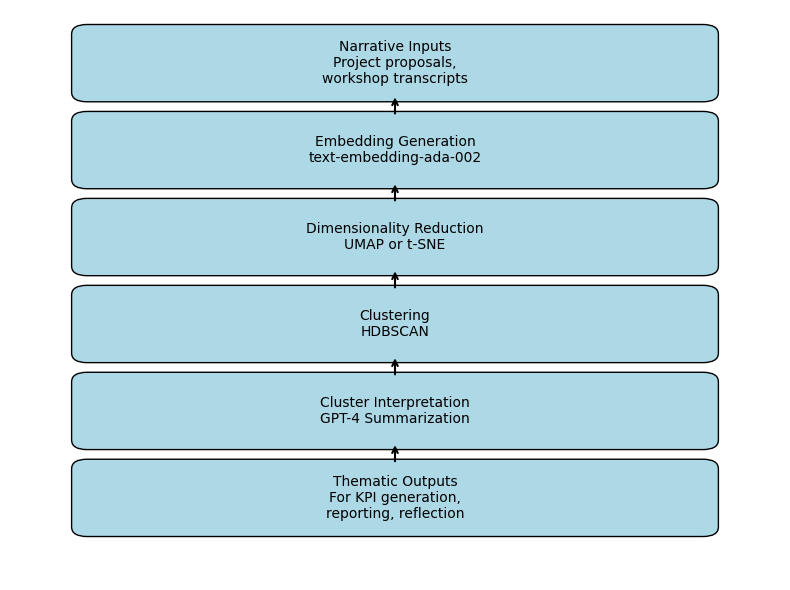
\includegraphics[width=0.9\textwidth]{../fig/clustering_pipeline}
    \caption{Semantic Clustering Pipeline for Narrative Inputs}
    \label{fig:clustering-pipeline}
\end{figure}

\subsection{KPI Derivation Pipeline}\label{subsec:kpi-pipeline}

The LangGraph pipeline enables auditable KPI generation:

\begin{enumerate}
    \item Input parsing and problem statement structuring
    \item Metric and leverage point extraction
    \item Solution mapping
    \item Impact framing using IOOI (Inputs, Outputs, Outcomes, Impact)
    \item SDG alignment
    \item Candidate indicator retrieval and critique
    \item KPI generation and audit loops
    \item Transparency trace logging
\end{enumerate}

\begin{figure}[H]
    \centering
    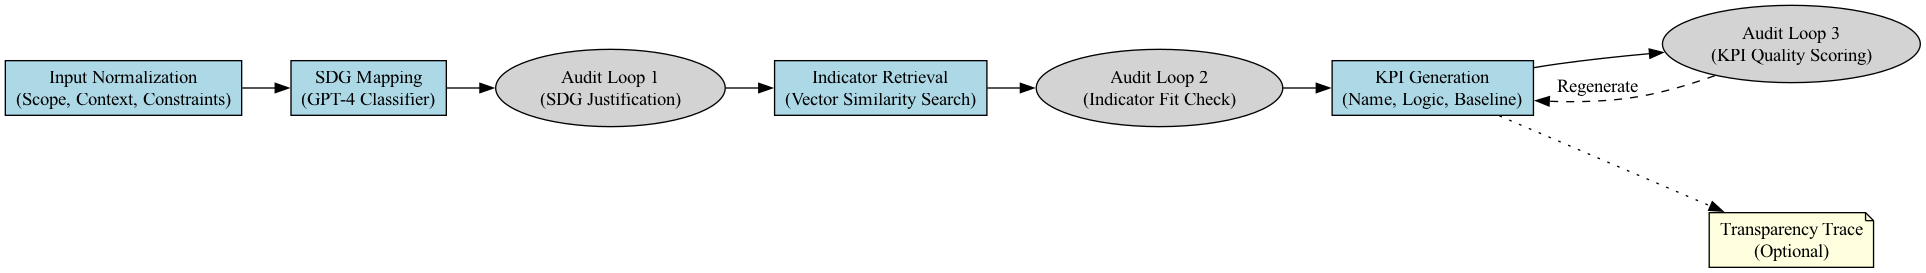
\includegraphics[height=0.9\textheight]{../fig/langgraph_pipeline}
    \caption{LangGraph Pipeline for KPI Derivation and Impact Structuring}
    \label{fig:langgraph-pipeline}
\end{figure}

\subsection{SDG Mapping and Justification}\label{subsec:sdg-mapping}

\begin{itemize}
    \item Projects are semantically classified against SDGs using GPT-4.
    \item Justification outputs provide transparency, enabling stakeholders to understand reasoning and challenge outputs if necessary.
\end{itemize}

\section{Integration with the Public Value Academy Platform}\label{sec:integration-platform}

The artefact was designed for seamless integration into the Public Value Academy digital infrastructure:

\begin{itemize}
    \item Supports workshops and guided reflection around public value.
    \item Enables iterative improvement of AI-supported evaluative tools.
    \item Embeds human-in-the-loop feedback directly into evaluation workflows.
\end{itemize}

\section{Ethical and Governance Considerations}\label{sec:ethical-governance}

\begin{itemize}
    \item GDPR-compliant handling of participant and project data.
    \item Explainable AI (XAI) principles applied throughout for transparency.
    \item Human oversight ensured in all critical stages (SDG mapping, KPI generation, indicator selection).
\end{itemize}

\section{Summary}\label{sec:artefact-summary}

Chapter 4 demonstrates that a prototypical, AI-supported IMM artefact can be designed to combine automated analysis with human judgment.
The artefact provides interpretable outputs, enables structured reflection on public value, and serves as the foundation for the demonstration and evaluation in the following chapter.